

\begin{center}
\thispagestyle{empty}
%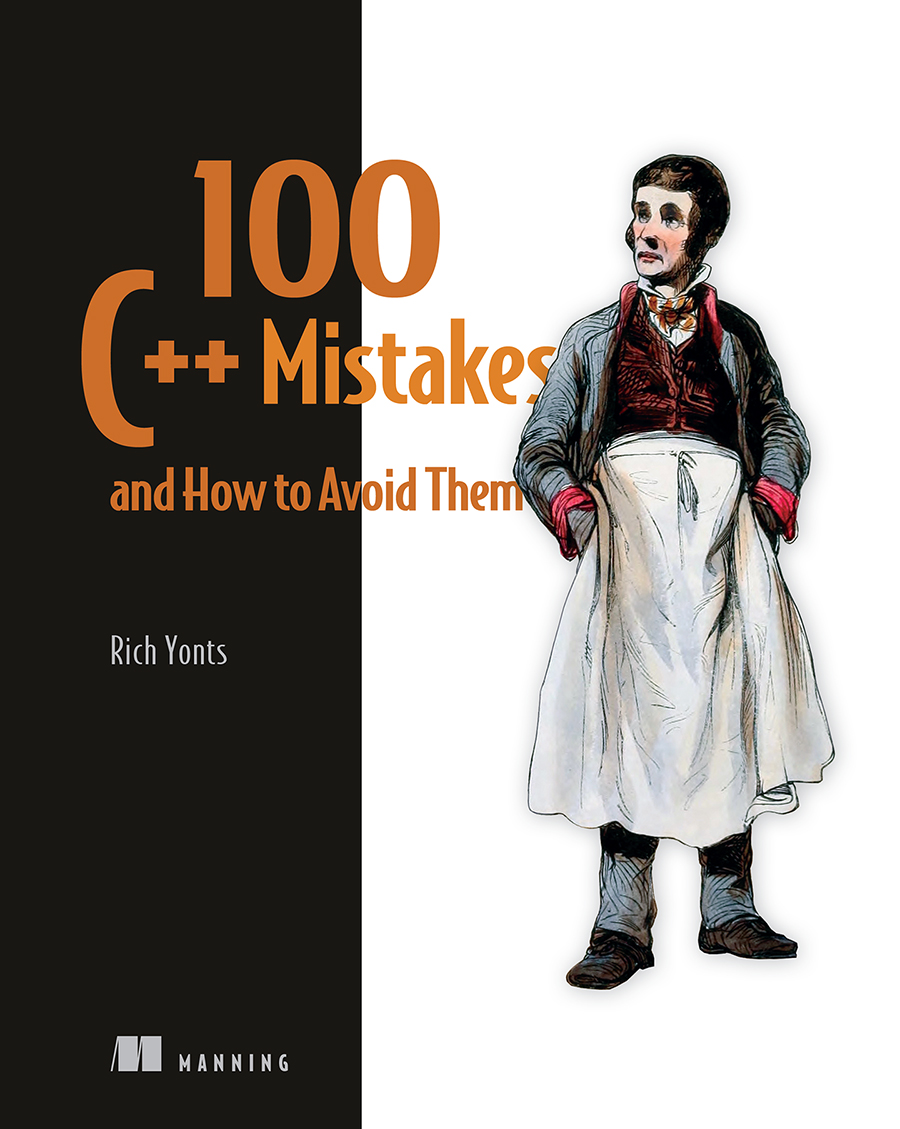
\includegraphics[width=\textwidth,height=\textheight,keepaspectratio]{cover.png}
\begin{tikzpicture}[remember picture, overlay, inner sep=0pt]
\node at (current page.center)
{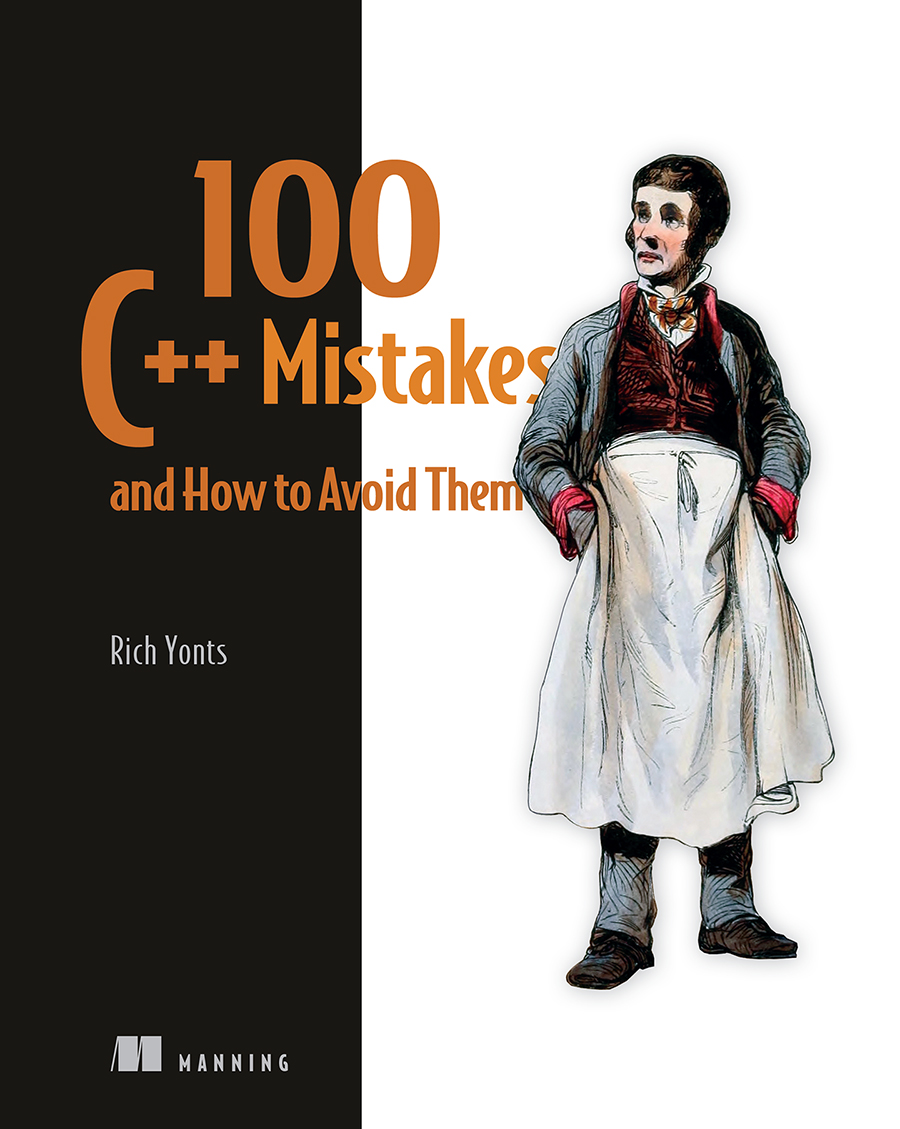
\includegraphics[width=\paperwidth, keepaspectratio=false]{cover.png}};
\end{tikzpicture}
\newpage
\thispagestyle{empty}
\huge
\textbf{C++编程避坑指南:100个常见错误及解决方案}
\\[9pt]
\normalsize
作者: Rich Yonts
\\[8pt]
\normalsize
译者:\href{https://github.com/xiaoweiChen/100-Cpp-Mistakes-and-How-to-Avoid-Them}{陈晓伟}
\\[8pt]
\end{center}

\newpage

\begin{comment}
\end{comment}

\myChapterNoContents{前言}{}{content/preface.tex}
\newpage

\myChapterNoContents{致谢}{}{content/acknowledgments.tex}
\newpage

\myChapterNoContents{关于本书}{}{content/about-this-book.tex}
\newpage

\myChapterNoContents{关于作者}{}{content/about-the-author.tex}
\newpage

\myChapterNoContents{封面插图}{}{content/about-the-cover-illustration.tex}
\newpage

\pagestyle{empty}
\tableofcontents
\newpage

\setsecnumdepth{section}

\myChapter{第1章}{C++:强大的控制力意味着重大的责任}{content/chapter1/0.tex}
\mySubsection{1.1.}{编程错误}{content/chapter1/1.tex}
\mySubsection{1.2.}{错误分析}{content/chapter1/2.tex}
\mySubsection{1.3.}{从错误中学习到了什么}{content/chapter1/3.tex}
\mySubsection{1.4.}{错误在哪里}{content/chapter1/4.tex}
\mySubsection{1.5.}{本书的结构}{content/chapter1/5.tex}
\mySubsection{1.6.}{总结}{content/chapter1/6.tex}
\newpage

\myPartGray{第一部分}{现代 C++}{content/part1/part.tex}
\newpage

\myChapter{第2章}{更好的现代C++:类和类型}{content/part1/chapter2/0.tex}
\mySubsection{2.1.}{Mistake 1: 没有使用移动语义}{content/part1/chapter2/1.tex}
\mySubsection{2.2.}{Mistake 2: 使用空异常规范}{content/part1/chapter2/2.tex}
\mySubsection{2.3.}{Mistake 3: 未对派生虚函数使用重写}{content/part1/chapter2/3.tex}
\mySubsection{2.4.}{Mistake 4: 编写简单的或隐藏不需要的提供类成员}{content/part1/chapter2/4.tex}
\mySubsection{2.5.}{Mistake 5: 不使用类内初始化器}{content/part1/chapter2/5.tex}
\mySubsection{2.6.}{Mistake 6: 过度使用基于索引的循环}{content/part1/chapter2/6.tex}
\mySubsection{2.7.}{Mistake 7: 不使使用nullptr}{content/part1/chapter2/7.tex}
\mySubsection{2.8.}{Mistake 8: 没有使用unique\_ptr来实现独占所有权}{content/part1/chapter2/8.tex}
\mySubsection{2.9.}{Mistake 9: 没有使用shared\_ptr来实现共享所有权}{content/part1/chapter2/9.tex}
\newpage

\myChapter{第3章}{更好的现代C++:通用编程}{content/part1/chapter3/0.tex}
\mySubsection{3.1.}{Mistake 10: 初始化时未能使用if}{content/part1/chapter3/1.tex}
\mySubsection{3.2.}{Mistake 11: 没有对变量使用类型推断}{content/part1/chapter3/2.tex}
\mySubsection{3.3.}{Mistake 12: 使用typedef}{content/part1/chapter3/3.tex}
\mySubsection{3.4.}{Mistake 13: 通用算法}{content/part1/chapter3/4.tex}
\mySubsection{3.5.}{Mistake 14: 不使用统一初始化}{content/part1/chapter3/5.tex}
\mySubsection{3.6.}{Mistake 15: 未使用就地初始化}{content/part1/chapter3/6.tex}
\mySubsection{3.7.}{Mistake 16: 未使用元组}{content/part1/chapter3/7.tex}
\mySubsection{3.8.}{Mistake 17: 不使用结构化绑定}{content/part1/chapter3/8.tex}
\newpage

\myChapter{第4章}{更好的现代C++:附加主题}{content/part1/chapter4/0.tex}
\mySubsection{4.1.}{Mistake 18: 不使用可变参数模板}{content/part1/chapter4/1.tex}
\mySubsection{4.2.}{Mistake 19: 使用全局命名空间枚举}{content/part1/chapter4/2.tex}
\mySubsection{4.3.}{Mistake 20: 不使用新的格式化功能}{content/part1/chapter4/3.tex}
\mySubsection{4.4.}{Mistake 21: 不使用容器的范围功能}{content/part1/chapter4/4.tex}
\mySubsection{4.5.}{Mistake 22: 编写非可移植的文件系统代码}{content/part1/chapter4/5.tex}
\mySubsection{4.6.}{Mistake 23: 编写过多的独立函数}{content/part1/chapter4/6.tex}
\mySubsection{4.7.}{Mistake 24: 使用笨拙的常量}{content/part1/chapter4/7.tex}
\mySubsection{4.8.}{Mistake 25: 编写模式匹配代码}{content/part1/chapter4/8.tex}
\newpage

\myPartGray{第二部分}{传统 C++}{content/part2/part.tex}
\newpage

\myChapter{第5章}{C语言的惯用法}{content/part2/chapter5/0.tex}
\mySubsection{5.1.}{Mistake 26: 总是在函数的顶部声明变量}{content/part2/chapter5/1.tex}
\mySubsection{5.2.}{Mistake 27: 依赖于宏}{content/part2/chapter5/2.tex}
\mySubsection{5.3.}{Mistake 28: 对于NULL的误解}{content/part2/chapter5/3.tex}
\mySubsection{5.4.}{Mistake 29: 使用FILE访问磁盘文件}{content/part2/chapter5/4.tex}
\mySubsection{5.5.}{Mistake 30: 将整数值转为布尔值}{content/part2/chapter5/5.tex}
\mySubsection{5.6.}{Mistake 31: 使用C风格的强制转换}{content/part2/chapter5/6.tex}
\mySubsection{5.7.}{Mistake 32: 使用atoi转换文本}{content/part2/chapter5/7.tex}
\mySubsection{5.8.}{Mistake 33: 使用C风格的字符串}{content/part2/chapter5/8.tex}
\mySubsection{5.9.}{Mistake 34: 调用exit函数}{content/part2/chapter5/9.tex}
\mySubsection{5.10.}{Mistake 35: 优先选择数组而非vector}{content/part2/chapter5/10.tex}
\newpage

\myChapter{第6章}{更好的前现代C++}{content/part2/chapter6/0.tex}
\mySubsection{6.1.}{Mistake 36: 使用 scanf 和 printf 进行输入和输出}{content/part2/chapter6/1.tex}
\mySubsection{6.2.}{Mistake 37: 过度使用 endl}{content/part2/chapter6/2.tex}
\mySubsection{6.3.}{Mistake 38: 使用 malloc 和 free 进行动态分配}{content/part2/chapter6/3.tex}
\mySubsection{6.4.}{Mistake 39: 使用联合(union)进行类型转换}{content/part2/chapter6/4.tex}
\mySubsection{6.5.}{Mistake 40: 使用 varargs 实现可变参数列表}{content/part2/chapter6/5.tex}
\mySubsection{6.6.}{Mistake 41: 类初始化顺序不正确}{content/part2/chapter6/6.tex}
\mySubsection{6.7.}{Mistake 42: 将非值类型添加到容器}{content/part2/chapter6/7.tex}
\mySubsection{6.8.}{Mistake 43: 推荐使用索引而非迭代器}{content/part2/chapter6/8.tex}
\newpage

\myPartGray{第三部分}{经典(前现代)C++}{content/part3/part.tex}
\newpage

\myChapter{第7章}{建立类不变量}{content/part3/chapter7/0.tex}
\mySubsection{7.1.}{类不变量确保类的正确设计}{content/part3/chapter7/1.tex}
\mySubsection{7.2.}{类设计中的错误}{content/part3/chapter7/2.tex}
\mySubsection{7.3.}{Mistake 44: 未能维护类不变量}{content/part3/chapter7/3.tex}
\mySubsection{7.4.}{Mistake 45: 没有将类视为数据类型}{content/part3/chapter7/4.tex}
\mySubsection{7.5.}{Mistake 46: 未为方法建立基础}{content/part3/chapter7/5.tex}
\mySubsection{7.6.}{Mistake 47: 未能实现“三大”函数}{content/part3/chapter7/6.tex}
\mySubsection{7.7.}{Mistake 48: 仅仅为了代码复用而使用继承}{content/part3/chapter7/7.tex}
\mySubsection{7.8.}{Mistake 49: 过度使用默认构造函数}{content/part3/chapter7/8.tex}
\mySubsection{7.9.}{Mistake 50: 未能维持"is-a"关系}{content/part3/chapter7/9.tex}
\newpage

\myChapter{第8章}{维持类不变量}{content/part3/chapter8/0.tex}
\mySubsection{8.1.}{维持类不变量}{content/part3/chapter8/1.tex}
\mySubsection{8.2.}{Mistake 51: 编写非必要的访问器方法}{content/part3/chapter8/2.tex}
\mySubsection{8.3.}{Mistake 52: 提供琐碎的修改器}{content/part3/chapter8/3.tex}
\mySubsection{8.4.}{Mistake 53: 过度使用受保护的实例变量}{content/part3/chapter8/4.tex}
\mySubsection{8.5.}{Mistake 54: 混淆operator=和复制构造函数的语义}{content/part3/chapter8/5.tex}
\mySubsection{8.6.}{Mistake 55: 误解浅复制与深复制语义}{content/part3/chapter8/6.tex}
\mySubsection{8.7.}{Mistake 56: 未能调用基类的操作符}{content/part3/chapter8/7.tex}
\mySubsection{8.8.}{Mistake 57: 未能在多态基类中使用虚析构函数}{content/part3/chapter8/8.tex}
\mySubsection{8.9.}{Mistake 58: 在构造函数和析构函数中调用虚函数}{content/part3/chapter8/9.tex}
\mySubsection{8.10.}{Mistake 59: 尝试使用多态数组元素}{content/part3/chapter8/10.tex}
\mySubsection{8.11.}{Mistake 60: 未能初始化所有实例变量}{content/part3/chapter8/11.tex}
\newpage

\myChapter{第9章}{类操作}{content/part3/chapter9/0.tex}
\mySubsection{9.1.}{Mistake 61: 对变量遮蔽的误解}{content/part3/chapter9/1.tex}
\mySubsection{9.2.}{Mistake 62: 允许复制唯一对象}{content/part3/chapter9/2.tex}
\mySubsection{9.3.}{Mistake 63: 未针对返回值优化进行编码}{content/part3/chapter9/3.tex}
\mySubsection{9.4.}{Mistake 64: 从复制赋值操作符不返回引用}{content/part3/chapter9/4.tex}
\mySubsection{9.5.}{Mistake 65: 忘记处理自我赋值}{content/part3/chapter9/5.tex}
\mySubsection{9.6.}{Mistake 66: 对前缀和后缀形式的误解}{content/part3/chapter9/6.tex}
\mySubsection{9.7.}{Mistake 67: 误导性的隐式转换操作符}{content/part3/chapter9/7.tex}
\mySubsection{9.8.}{Mistake 68: 过度使用隐式转换构造函数}{content/part3/chapter9/8.tex}
\mySubsection{9.9.}{Mistake 69: 过于关注独立操作符}{content/part3/chapter9/9.tex}
\mySubsection{9.10.}{Mistake 70: 未能将非变异方法标记为常量}{content/part3/chapter9/10.tex}
\mySubsection{9.11.}{Mistake 71: 未能正确地标记类方法为静态}{content/part3/chapter9/11.tex}
\mySubsection{9.12.}{Mistake 72: 在选择成员函数和非成员函数之间做出错误决定}{content/part3/chapter9/12.tex}
\mySubsection{9.13.}{Mistake 73: 从访问器方法中错误地返回字符串}{content/part3/chapter9/13.tex}
\newpage

\myChapter{第10章}{异常与资源管理}{content/part3/chapter10/0.tex}
\mySubsection{10.1.}{使用异常}{content/part3/chapter10/1.tex}
\mySubsection{10.2.}{Mistake 74: 不在构造函数中抛出异常}{content/part3/chapter10/2.tex}
\mySubsection{10.3.}{Mistake 75: 从析构函数中抛出异常}{content/part3/chapter10/3.tex}
\mySubsection{10.4.}{Mistake 76: 使用异常时允许资源泄漏}{content/part3/chapter10/4.tex}
\mySubsection{10.5.}{Mistake 77: 未能使用RAII模式}{content/part3/chapter10/5.tex}
\mySubsection{10.6.}{Mistake 78: 使用原始指针管理资源}{content/part3/chapter10/6.tex}
\mySubsection{10.7.}{Mistake 79: 混合使用new和delete的不同形式}{content/part3/chapter10/7.tex}
\mySubsection{10.8.}{Mistake 80: 信任异常说明}{content/part3/chapter10/8.tex}
\mySubsection{10.9.}{Mistake 81: 未能通过值抛出并通过引用捕获}{content/part3/chapter10/9.tex}
\newpage

\myChapter{第11章}{函数与编码}{content/part3/chapter11/0.tex}
\mySubsection{11.1.}{设计考量}{content/part3/chapter11/1.tex}
\mySubsection{11.2.}{Mistake 82: 使用重载函数而不是参数默认值}{content/part3/chapter11/2.tex}
\mySubsection{11.3.}{Mistake 83: 未能使用断言}{content/part3/chapter11/3.tex}
\mySubsection{11.4.}{Mistake 84: 返回指向局部对象的指针或引用}{content/part3/chapter11/4.tex}
\mySubsection{11.5.}{Mistake 85: 使用输出参数}{content/part3/chapter11/5.tex}
\mySubsection{11.6.}{Mistake 86: 参数类型的不正确使用}{content/part3/chapter11/6.tex}
\mySubsection{11.7.}{Mistake 87: 依赖参数求值顺序}{content/part3/chapter11/7.tex}
\mySubsection{11.8.}{Mistake 88: 传递过多参数}{content/part3/chapter11/8.tex}
\mySubsection{11.9.}{Mistake 89: 函数过长且包含多种行为}{content/part3/chapter11/9.tex}
\mySubsection{11.10.}{Mistake 90: 职能过多的函数}{content/part3/chapter11/10.tex}
\newpage

\myChapter{第12章}{通用编码}{content/part3/chapter12/0.tex}
\mySubsection{12.1.}{Mistake 91: 不正确处理除以零}{content/part3/chapter12/1.tex}
\mySubsection{12.2.}{Mistake 92: 不正确地使用循环中的continue关键字}{content/part3/chapter12/2.tex}
\mySubsection{12.3.}{Mistake 93: 未能将已删除的指针设置为NULL}{content/part3/chapter12/3.tex}
\mySubsection{12.4.}{Mistake 94: 未能直接返回计算得到的布尔值}{content/part3/chapter12/4.tex}
\mySubsection{12.5.}{Mistake 95: 对表达式的利用不足}{content/part3/chapter12/5.tex}
\mySubsection{12.6.}{Mistake 96: 使用多余的else关键字}{content/part3/chapter12/6.tex}
\mySubsection{12.7.}{Mistake 97: 不使用辅助函数}{content/part3/chapter12/7.tex}
\mySubsection{12.8.}{Mistake 98: 错误地比较浮点数值}{content/part3/chapter12/8.tex}
\mySubsection{12.9.}{Mistake 99: 浮点数到整数的赋值}{content/part3/chapter12/9.tex}
\mySubsection{12.10.}{Mistake 100: 忽略编译器警告}{content/part3/chapter12/10.tex}
\newpage

\begin{comment}
\end{comment}
